%!TEX root = ../../thesis.tex

\section{A Brief History of Open-domain QA}
\label{sec:openqa-rw}

Question answering was one of the earliest tasks for NLP systems since 1960s. One early system, which prefigures modern text-based question answering systems, was the \sys{Protosynthex} system of \cite{simmons1964indexing}. The system first formulated a query based on the content words in the question, retrieved candidate answer sentences based on the frequency-weighted term overlap with the question, and finally performed a dependency parse match to get the final answer. Another notable system \sys{MURAX} \cite{kupiec1993murax}, was designed to answer general-knowledge questions over \sys{Grolier}'s on-line encyclopedia, using shallow linguistic processing and information retrieval (IR) techniques.

The interest in open domain question answering has increased since 1999, when the QA track was first included as part of the annual TREC competitions\footnote{\url{http://trec.nist.gov/data/qamain.html}}. The task was at first defined such that the systems were to retrieve small snippets of text that contained an answer for open-domain questions. It has spurred a wide range of QA systems developed at the time, and the majority of the systems consisted of two stages: an IR system used to select the top $n$ documents or passages which match a query that has been generated from the question, and a window-based word scoring system used to pinpoint likely answers. For more details, readers are referred to \cite{voorhees1999trec,moldovan2000structure}.

More recently, with the development of knowledge bases (KBs) such as \sys{Freebase}~\cite{bollacker2008freebase} and \sys{DBpedia}~\cite{auer2007dbpedia}, many innovations have occurred in the context of question answering from KBs with the creation of resources like \sys{WebQuestions} \cite{berant2013semantic} and \sys{SimpleQuestions} \cite{bordes2015large} based on \sys{Freebase}, or on automatically extracted KBs, e.g., OpenIE triples and \sys{NELL} \cite{fader2014open}. A lot of progress has been made on knowledge-based question answering and the major approaches are either based on semantic parsing or information extraction techniques~\cite{yao2014freebase}. However, KBs have inherent limitations (incompleteness and fixed schemas) that motivated researchers to return to the original setting of answering from raw text lately.

\begin{figure}[t]
    \center
    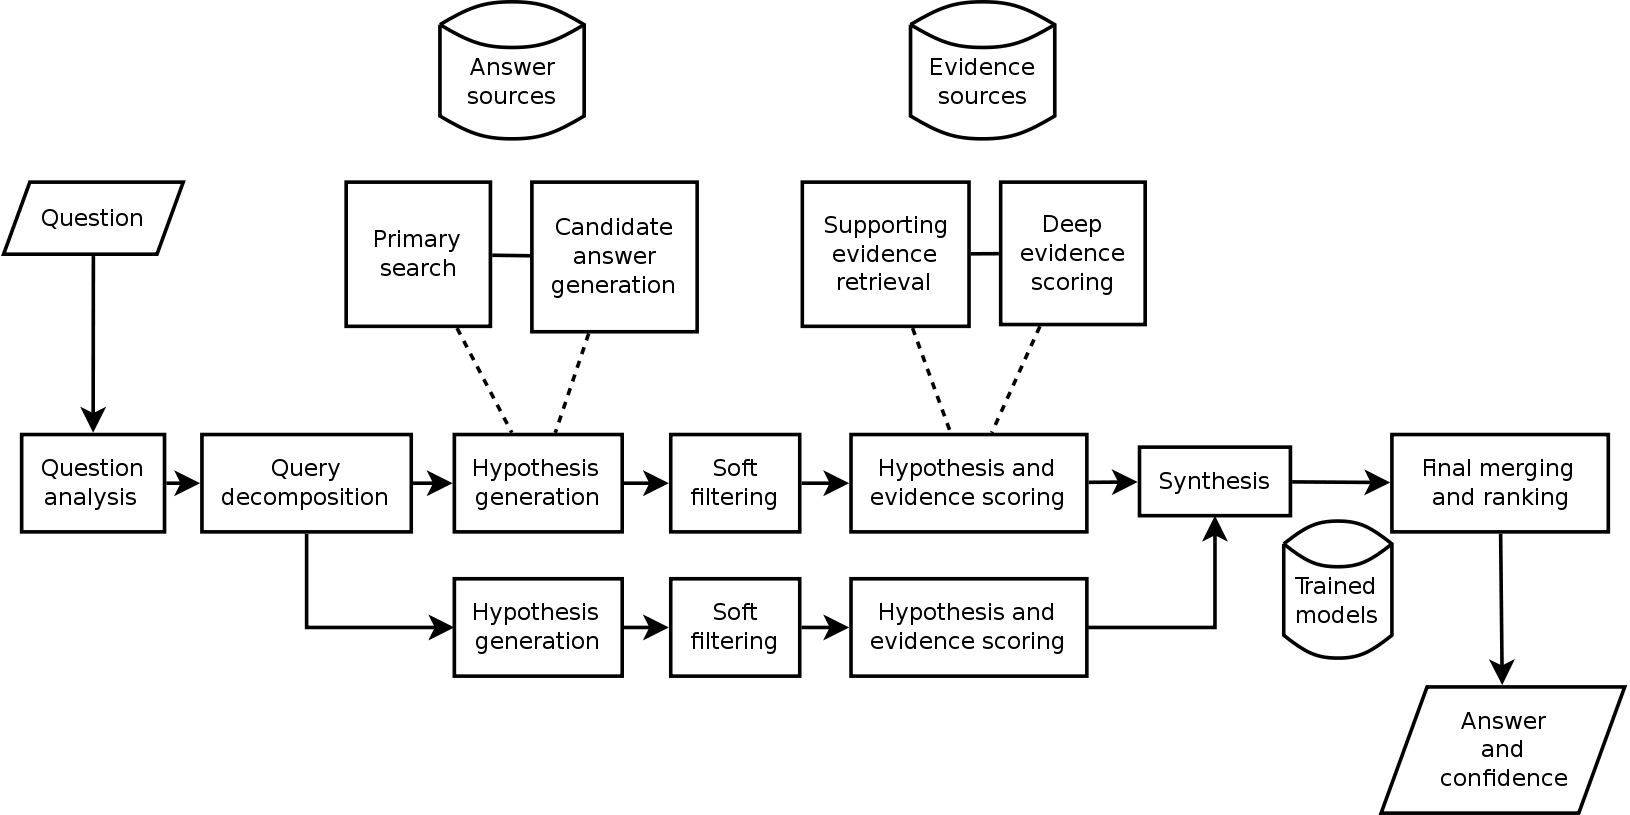
\includegraphics[scale=0.25]{img/deepqa.png}
    \longcaption{The high-level architecture of IBM's \sys{DeepQA} used in \sys{Watson}.}{\label{fig:watson}The high-level architecture of IBM's \sys{DeepQA} used in \sys{Watson}. Image courtesy: \href{https://en.wikipedia.org/wiki/Watson_(computer)}{https://en.wikipedia.org/wiki/Watson\_(computer)}.}
\end{figure}

There are also a number of highly developed full pipeline QA approaches using a myriad of resources, including both text collections (Web pages, Wikipedia, newswire articles) and structured knowledge bases (\sys{Freebase}, \sys{DBpedia} etc.). A few notable systems include Microsoft's \sys{AskMSR} \cite{brill2002askmsr},
IBM's \sys{DeepQA} \cite{ferrucci2010building} and \sys{YodaQA} \cite{baudivs2015yodaqa} --- the latter of which is open source and hence reproducible for comparison purposes. \sys{AskMSR} is a search-engine based QA system that relies on ``data redundancy rather than sophisticated linguistic analyses of either questions or candidate answers''. \sys{DeepQA} is the most representative modern question answering system and its victory at the TV game-show \sys{Jeopardy!} in 2011 received a great deal of attention. It is a very sophisticated system that consists of many different pieces in the pipeline and it relies on unstructured information as well as structured data to generate candidate answers or vote over evidence. A high-level architecture is illustrated in Figure~\ref{fig:watson}. \sys{YodaQA} is an open source system modeled after \sys{DeepQA}, similarly combining websites, databases and Wikipedia in particular. Comparing against these methods provides a useful datapoint for an ``upper bound'' benchmark on performance.

Finally, there are other types of question answering problems based on different types of resources, including Web tables~\cite{pasupat2015compositional}, images~\cite{antol2015vqa}, diagrams~\cite{kembhavi2017you} or even videos~\cite{tapaswi2016movieqa}. We are not going into further details as our work focuses on text-based question answering.

Our \sys{DrQA} system (Section~\ref{sec:drqa}) focuses on question answering using Wikipedia as the unique knowledge source, such as one does when looking for answers in an encyclopedia.  QA using Wikipedia as a resource has been explored previously. \newcite{ryu2014open} perform open-domain QA using a Wikipedia-based knowledge model. They combine article content with multiple other answer matching modules based on different types of semi-structured knowledge such as infoboxes, article structure, category structure, and definitions. Similarly, \newcite{Ahn2004using} also combine Wikipedia as a text resource with other resources, in this case with information retrieval over other documents. \newcite{buscaldi2006mining} also mine knowledge from Wikipedia for QA. Instead of using it as a resource for seeking answers to questions, they focus on validating answers returned by their QA system, and use Wikipedia categories for determining a set of patterns that should fit with the expected answer. In our work, we consider the comprehension of text only, and use Wikipedia text documents as the sole resource in order to emphasize the task of reading comprehension. We believe that adding other knowledge sources or information will further improve the performance of our system.
